%%%%%%%%%%%%%%%%%%%% author.tex %%%%%%%%%%%%%%%%%%%%%%%%%%%%%%%%%%%
%
% sample root file for your "contribution" to a contributed volume
%
% Use this file as a template for your own input.
%
%%%%%%%%%%%%%%%% Springer %%%%%%%%%%%%%%%%%%%%%%%%%%%%%%%%%%%%%%%%%


% RECOMMENDED %%%%%%%%%%%%%%%%%%%%%%%%%%%%%%%%%%%%%%%%%%%%%%%%%%%
\documentclass[graybox]{svmult}

% choose options for [] as required from the list
% in the Reference Guide

\usepackage{mathptmx}       % selects Times Roman as basic font
\usepackage{helvet}         % selects Helvetica as sans-serif font
\usepackage{courier}        % selects Courier as typewriter font
\usepackage{type1cm}        % activate if the above 3 fonts are
                             % not available on your system

\usepackage{makeidx}         % allows index generation
\usepackage{graphicx}        % standard LaTeX graphics tool
                             % when including figure files
\usepackage{multicol}        % used for the two-column index
\usepackage[bottom]{footmisc}% places footnotes at page bottom

\usepackage{amsthm}
\newtheorem{mydef}{Definition}

% see the list of further useful packages
% in the Reference Guide

\makeindex             % used for the subject index
                       % please use the style svind.ist with
                       % your makeindex program

%%%%%%%%%%%%%%%%%%%%%%%%%%%%%%%%%%%%%%%%%%%%%%%%%%%%%%%%%%%%%%%%%%%%%%%%%%%%%%%%%%%%%%%%%

\begin{document}

\title{Extraction of Software Product Line Architectures from Many System Variants}
% Use \titlerunning{Short Title} for an abbreviated version of
% your contribution title if the original one is too long
\author{Anas Shatnawi, Abdelhak Seriai and Houari Sahraoui}
% Use \authorrunning{Short Title} for an abbreviated version of
% your contribution title if the original one is too long

\institute{Anas Shatnawi \at Sorbonne University, CNRS, LIP6, F-75005 Paris, France. \email{shatnawi@lip6.fr}
\and Abdelhak Seriai \at University of Montpellier, CNRS, LIRMM, Montpellier, France. \email{seriai@lirmm.fr}
\and Houari Sahraoui \at University of Montreal, GEODES, Montreal, Quebec, Canada. \email{sahraouh@iro.umontreal.ca}}
%
% Use the package "url.sty" to avoid
% problems with special characters
% used in your e-mail or web address
%
\maketitle

%\abstract*{Abstract.}

\abstract{
Software Product Line Architecture (SPLA) describes the architecture of a set of software variants by describing (i) what components can be included in the product configuration based on the selected features of this product (ii) how these components can be configured to form a concrete architecture of the product, (iii) shared components, and (vi) individual architecture characteristics of each product. However, developing SPLA from scratch is known a highly, costly and risky task. The alternative is to exploit the already developed \emph{legacy} software variants to reverse engineer SPLA. This reduces the cost of Software Product Line (SPL) development and allows to manage software variants as a SPL. 
In this chapter, we discuss the extraction of SPLA based on the analysis of several software variants. 
Precisely, we discuss the variability in SPLA. Then, we discuss challenges in extracting variability of SPLA and highlight a number of good practices proposed in the-state-of-the-art of the SPLA extraction. Next, we discuss one example approach that completely extracts SPLA of software variants.}


\section{Introduction}
\label{sec:1:intro}
Software Product Line Architecture (SPLA) represents one of the most important software elements of a Software Product Line (SPL). In the literature, many definitions have been proposed for SPLA. These definitions consider SPLA as a core architecture that captures the variability of a set of software products at the architecture level. However, they differ in terms of the variability definition. For instance, DeBaud et al. \cite{debaud1998pulse} defined  SPLA as an architecture shared by their member products and has such a variability degree. This is a very general definition since it does not specify the nature of the architecture variability. In contrast, Pohl et al. \cite{3_pohl2005software} provide a more precise definition by specifying the nature of architecture variability. In this definition, SPLA includes variation points and variants that are presented in such a variability model. Gomaa \cite{Gomaa} links the architecture variability with the architectural-elements. Thus, in his definition, SPLA describes the variability in terms of mandatory, optional, and variable components, and their connections. As a synthesis of these definitions, we propose the following one:

\begin{mydef}
\textbf{Software Product Line Architecture (SPLA)} describes the high level structures, and the commonality and the variability related to components and architectural configuration of a set of software variants of a SPL. \index{Software Product Line Architecture}
\end{mydef}

Companies rely on three approaches to develop SPLA of a SPL: \textit{proactive}, \textit{reactive} and \textit{extractive} \cite{gasparic2014analysis,shatnawi2017recovering}.

\begin{itemize}
\item \textbf{Proactive approach:} companies develop SPLA from scratch. They need to understand the commonality and the variability of the SPL in advance. However, developing SPLA from scratch is known to be a highly costly and risky task.
\index{Proactive approach}

\item \textbf{Reactive approach:} companies incrementally develop SPLA during the development of a SPL. This can reduce the cost and the risk compared to the proactive strategy. \index{Reactive approach}

\item \textbf{Extractive approach:} companies exploit the already developed \emph{legacy} software variants to reverse engineer SPLA. This is based on the analysis of the commonality and the variability between the software artifacts of software variants to extract the SPLA. This allows companies to significantly reduce the cost of SPLA development compared to the proactive and reactive approaches. The Extractive approach was used by 50\% of companies according to the industrial survey of SPL adaptation \cite{berger2013survey}. \index{Extractive approach}
\end{itemize}

In many cases, companies usually develop several software variants with functional and technical variations without using SPLs \cite{dubinsky2013exploratory,fischer2014enhancing}. In their recent studies, Fischer et al. \cite{fischer2014enhancing} reported that it becomes an industrial practice to rely on the \textit{clone-and-own} approach to develop similar software variants based on copying functionalities from existing software variants and by customizing these functionalities to meet the varied requirements of new customers \cite{fischer2014enhancing}. Nevertheless, managing the software reuse and maintenance of these software variants and their cloned functionalities is a very hard task when the number of software variants is increased \cite{dubinsky2013exploratory}. Therefore, it is important to systematically manage the commonality and variability between software variants using SPLs. One of the main challenges is to manage the commonality and variability between software variants at the architecture level by extracting SPLA. \index{Software variants}


In this chapter, we discuss the extraction of SPLA based on the analysis of several software variants. {We present an illustrative example in Section \ref{sec:ilstrativeexample}.}
We discuss the variability in SPLA in Section \ref{sec:variability-spla}, including the different types of SPLA variability. 
Next, we discuss challenges concerning the extraction of SPLA from many software variants in Section \ref{sec-challanges}. 
Then, in Section \ref{sec:extraction-spla}, we discuss the process of SPLA extraction and highlight a number of good practices of this extraction. Next, to illustrate the whole extraction process, we present an approach that completely identifies SPLA of software variants in Section \ref{sec:example-approach}. Finally, we conclude the chapter in Section \ref{sec:conclusion}.

\begin{figure}[b!]
\centering
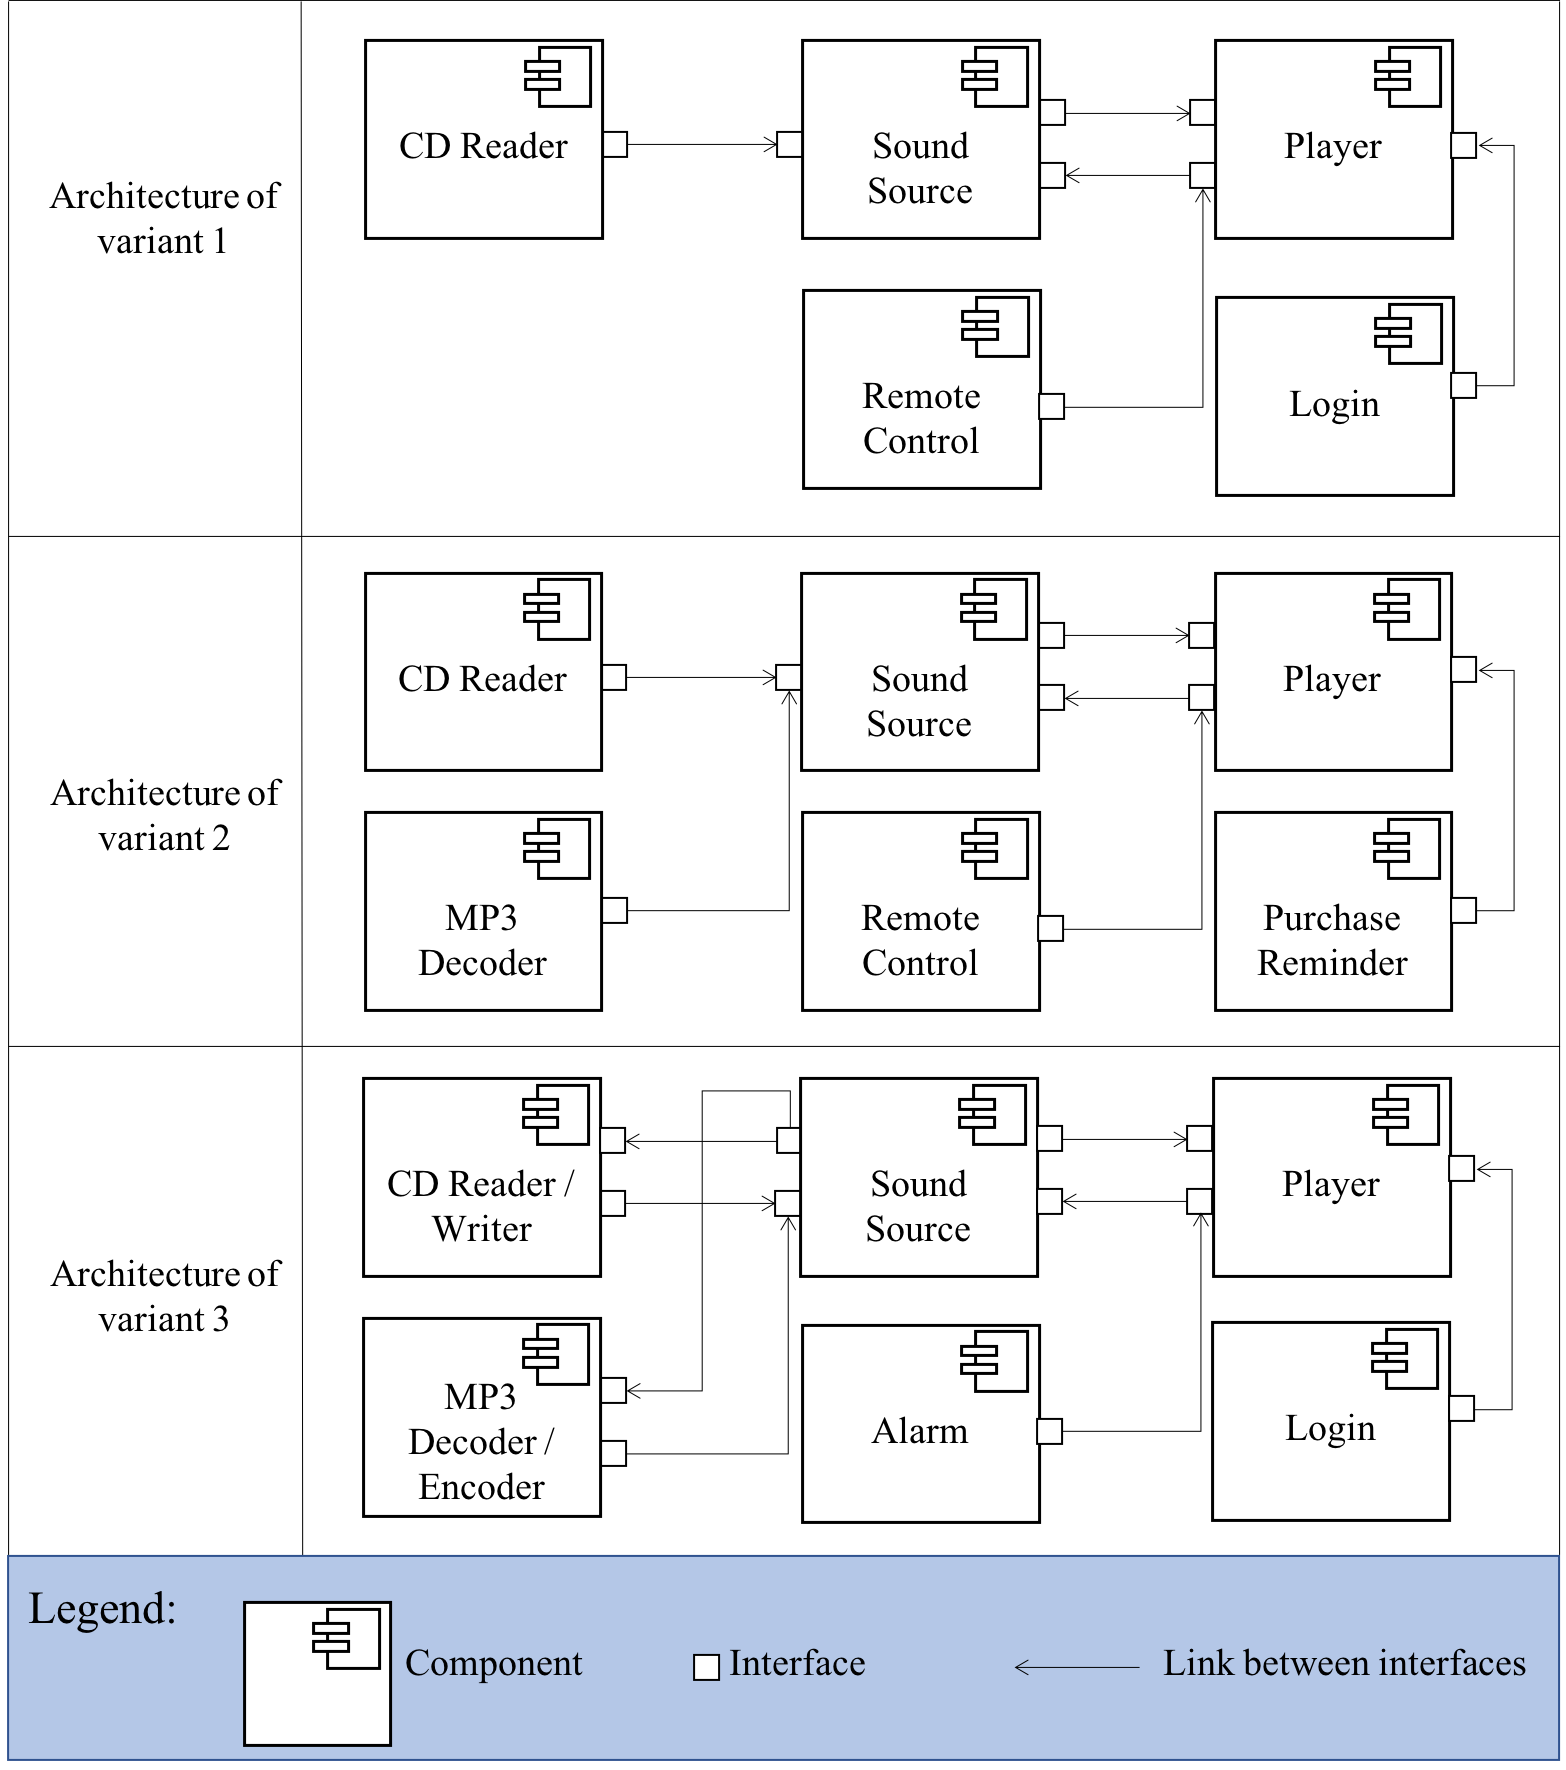
\includegraphics[width=\textwidth]{figs/kind_architecture_variability.png}
\caption{An illustrative example of architecture variability}
\label{fig:archVarExam1}
\end{figure}

\section{An Illustrative Example}
\label{sec:ilstrativeexample}
\index{Illustrative example}
We provide an illustrative example presented in Figure \ref{fig:archVarExam1} to better understand the architecture variability of software variants. This example includes the architecture of three software variants from the audio player software family.
The first software architecture consists of five components: \textit{CD Reader}, \textit{Sound Source}, \textit{Player}, \textit{Login} and  \textit{Remote Control} components. The second software architecture contains six components: \textit{CD Reader}, \textit{Sound Source}, \textit{Player}, \textit{Remote Control}, \textit{MP3 Decoder} and \textit{Purchase Reminder}. The third software architecture has six components: \textit{CD Reader}, \textit{Sound Source}, \textit{Player}, \textit{MP3 Decoder}, \textit{Login} and \textit{Alarm}. 

To show different types of variability in SPLA, we include diversity related to the components composing each architecture, the functionalities implemented by the same component in different software variants (\textit{MP3 Decoder} and \textit{MP3 Decoder/Encoder}), the interfaces (provided and required) of components and the links between these components.



\section{Variability in SPLA}
\label{sec:variability-spla}

\index{Variability in SPLA}


The main theme of software product line engineering is software variability. It concerns the \textit{susceptibility} and \textit{flexibility} of software to change to meet the needs of different customers \cite{1_clements2002}. The variability exists at \textit{different levels of abstraction} of the development life cycle of software variants of a SPL (e.g. requirement, design, implementation) \cite{1_clements2002}.
At the \textit{requirement level}, the variability is instituted from the \textit{diversity in customers' wishes}. Each customer selects a different set of features to be included in the software variant. In the illustrative example, the customer of the first software variant selects \textit{CD Reader} and one of the third software variant selects \textit{CD Reader}, and \textit{CD Writer} features. This variability is documented by the feature modeling language in most cases \cite{7_kang1990feature}.  This variability at the requirement level \textit{does not carry technical concerns} \cite{3_pohl2005software}.  Starting from the\textit{ design level}, the variability has more details concerning \textit{technical solutions about how to implement the features to form the software architectures}. It describes how the variability is built and implemented with regard to the point of view of software architects \cite{3_pohl2005software}. The technical variability details concerns \textit{what software components are included in the software architecture} (e.g., \textit{CD Reader}, \textit{Sound Source} and \textit{Player} components), \textit{how these components interact through their interfaces} (e.g., \textit{CD Reader} provides a sound stream interface to \textit{Sound Source}), and \textit{what topology forms the architectural configuration} (i.e. how components are composed) \cite{nakagawa2011reference}. SPLA should describe all these technical details \cite{shatnawi2017recovering}. 

SPLA explores the commonality and the variability of the architectural elements, i.e. \textit{component}, \textit{connector} and \textit{configuration} variability to realize the architecture variability. We will exclude connector variability because most of the architecture description languages such as \cite{canal1999specification,luckham1996rapide,magee1996dynamic} do not take the connectors as first class concepts. This means that we will only focus on component and configuration variability. Therefore, SPLA should describe \textit{component variability}, \textit{configuration variability} and \textit{dependencies between the components}.

\subsection{Component Variability}
\index{Component variability}

Components represent the main building elements of the software architecture that define the functionalities of the corresponding software. 
The component variability starts from the existence of many software components that have the same architectural meaning in terms of their implemented functionalities compared to the big picture of the software architectures of several software variants. \textit{MP3 Decoder} and \textit{MP3 Decoder/Encoder} are examples of these components in Figure \ref{fig:archVarExam1}. We call these similar software components as \textit{component variants} and we define them as follows: 

\begin{mydef}
\textbf{Component variants} {are a collection of components that have  the same   architectural meaning across software variants by offering the same features with technical or functional variations.}
\end{mydef} \index{Component variants}



We also need to enable capturing the commonality and the variability between component variants to understand the similarities and differences in their  implemented functionalities. This requires to provide a mechanism to identify the \textit{{structure} variability} and the \textit{{interface} variability}.


Component {structure} variability concerns the differences compared to the implementation details of component variants. This is related to the variability in the set of functionalities (e.g., \textit{Decoder} or \textit{Decoder/Encoder}) implemented by these component variants. This component structure variability can be presented at the class, method, attribute or even statement levels. The choice of the level is left to software architects. We should identify the \textit{common elements} that belong to all component variants, and the \textit{variable elements} that do not belong to all component variants. We define component structure variability as follows:

\begin{mydef}
\textbf{Component {structure} variability} concerns the differences in the structure of the component variants identified at the implementation level. 
\end{mydef}

\index{Component structure variability}


Component {interface} variability is related to the interaction between component variants with other components in different architectures. This is based on the variability in the component interfaces: provided and required ones. 
Each component provided interface provides an abstract description to access the functionalities of the component based on a set of method invocations. Component variants could be variable in their provided interfaces in the different software variants. In Figure \ref{fig:interVarEx}, \textit{CD Reader} and \textit{CD Reader/Writer} are component variants that are variable in their interfaces. \textit{CD Reader} provides a single interface to read the \textit{CD} content, while \textit{CD Reader/Writer} has an additional required interface related to the additional functionalities of writing on a CD that requires a source of information. We need to distinguish between mandatory and optional interfaces. Mandatory interfaces exist in all component variants. Optional interfaces exist in some component variants. We define component interface variability as follows:

\begin{mydef}
\textbf{Component {interface} variability} is the interaction variability between components through their provided and required interfaces.
\end{mydef}
\index{Component interface variability}


\begin{figure}[h]
\centering
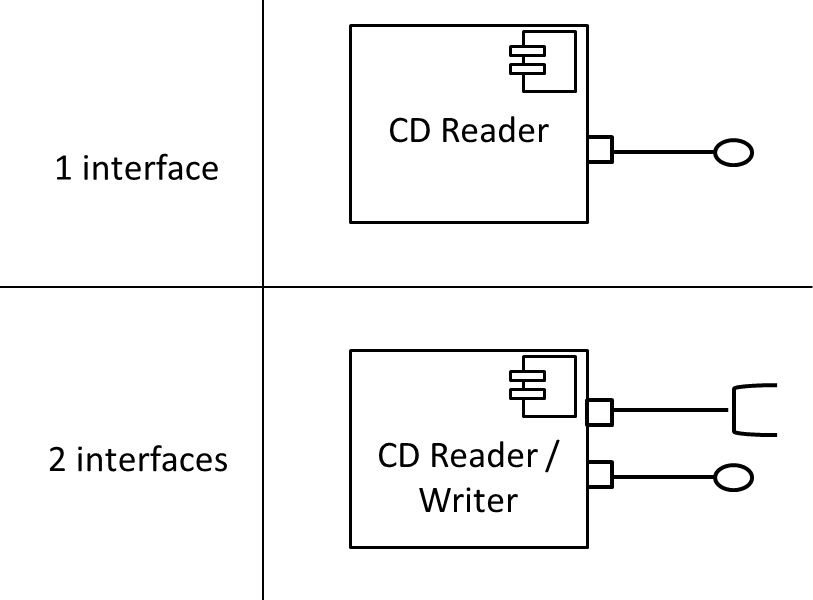
\includegraphics[width=0.5\textwidth]{figs/interfaceVarExample.png}
\caption{An example of variability of two component variants}
\label{fig:interVarEx}
\end{figure}


\subsection{ {Architecture} Configuration Variability} 
\index{Configuration variability}
The architectural configuration defines the collection of software components to be included in the software architecture, and the topology of how components are linked through their interfaces. Therefore, the configuration variability is represented in terms of the \textit{component existence variability}, as well as the \textit{component-to-component link variability}. We define configuration variability as follows:

\begin{mydef}
\textbf{Configuration variability} determines the mandatory and optional components as well as the  mandatory and optional component-to-component links to be included in different architectures of software variants.
\end{mydef}


Component existence variability concerns the presence and absence of components in the software architectures of different software variants. We define this variability in terms of the collection of \textit{mandatory} and \textit{optional} components. Mandatory components should be included in any software architecture of software variants. Optional components are not mandatory to be included in the software architecture of a software variant. In the illustrative example in Figure \ref{fig:archVarExam1}, \textit{Sound Source} is a mandatory component because it is a part of all software architectures, and \textit{Purchase Reminder} is an optional component because it is only a part of the second software architecture. We define component existence variability as follows:

\index{Component existence variability}

\begin{mydef}
\textbf{Component existence variability}  {refers to the mandatory or optional existence of a given component in the architecture of a specific software variant.}
\end{mydef}


The component-to-component link is the connection of two components based on their interfaces. With variability, a component can be linked with various components in different software variants. A component could be linked with a group of components in one software variant, and it could be linked with a different group of components in other software variants. In Figure \ref{fig:archVarExam1}, we show an example of component-to-component link variability where \textit{CD Reader} has only one link with \textit{Sound Source} in the first and the second software architectures, while \textit{CD Reader} has two links with \textit{Sound Source} and \textit{MP3 Decoder/Encoder} in the third software architecture.

 
The component-to-component link variability is related to the \textit{component existence variability}. For instance, the existence of a link between \textit{CD Reader} and \textit{MP3 Decoder/Encoder} is related to the selection of \textit{CD Reader} and \textit{MP3 Decoder/Encoder} in the architecture of software variant. Therefore, we consider a component-to-component link as a mandatory link if and only if it occurs in the architecture as well as the connected components are included in the architecture. Otherwise, it is considered as optional component-to-component link. We define component-to-component link variability as follows:

\index{Component-to-component link variability}

\begin{mydef}
\textbf{Component-to-component link variability}  {refers to the mandatory or optional existence of a particular link between two components, i.e., interface connection, in the architecture of a specific software variant as well as the corresponding components are included in the architecture of this software variant.}
\end{mydef}



 \subsection{Component dependencies}

\index{Component dependencies}

The component and configuration variabilities, discussed earlier, are not enough to define a valid architecture of a software variant. We also need the  dependencies, i.e. constraints, between components. Such dependencies are related to the feature variability. They can be of five types: \textit{Require}, \textit{And},  \textit{Exclude}, \textit{Alternative}, and \textit{Or} dependencies between the components \cite{shatnawi2017recovering}. We define these dependencies as follows:
    
  \index{Required dependency}  
\begin{mydef}
\textbf{Required dependency} refers to the necessary selection of a component to select another one; i.e. \textit{Component B} is required to select \textit{Component A}.
\end{mydef}

\index{And dependency}
\begin{mydef}
\textbf{And dependency} is the bidirectional form of the required one; i.e. \textit{Component A} requires \textit{Component B} and vice versa. More generally, the selection of one component among a set of components requires the selection of all the other components.
\end{mydef}

\index{Exclude dependency}
\begin{mydef}
\textbf{Exclude dependency} refers to the antagonistic relationship; i.e. \textit{Component A} and \textit{Component B} cannot occur in the same architecture.
\end{mydef}

\index{Alternative dependency}
\begin{mydef}
\textbf{Alternative dependency} generalizes the exclude one by exclusively selecting only one component from a set of components.
\end{mydef}

\index{Or dependency}
\begin{mydef}
\textbf{Or dependency} refers to the obligation to select at least one component between a set of components to be included in a software variant. 
\end{mydef}

To better understand a large number of \textit{Require}, \textit{And},  \textit{Exclude}, \textit{Alternative}, and \textit{Or} dependencies between different components, we analyze these dependencies to identify their relationships in terms of \textit{groups of variability}. Such relationships are the overlapping between dependencies. 
Several dependencies are the constraints of a common set of components. For example, a component has an \textit{Or} dependency with components having \textit{And} dependencies among themselves. We represent these dependencies using a hierarchical tree (e.g. feature model of components) to help support software architects to perform their tasks. We define groups of variability as follows:

\index{Groups of variability}
\index{Component feature model}
\begin{mydef}
\textbf{Groups of variability} organizes the overlapping of dependencies between components based on a feature model of components. 
\end{mydef}



\section{Challenges in Extracting SPLA from Software Variants}
\label{sec-challanges}
\index{Challenges in extracting SPLA}
In the previous section, we defined the SPLA and explained the different types of variability of architectural elements of the SPLA. In this section, we discuss challenges related to the extraction of SPLA based on the analysis of many software variants. 

Unlike the extraction of the software architecture of single software, the extraction of SPLA from multiple software variants requires the analysis of all these software variants. In most cases, these software variants are developed using the clone-and-own approach in an ad-hoc manner. Meaning, the cloning of software variants from existing ones is done without preserving contorting the commonalty and the variability across software variants. That makes the comparison of software artifacts of different software variants hard due to the loss of the architectures of some software variants because there is no a rigorous coordination process to enforce the development teams to provide architectures of their software variants with respect to the previously developed software variants. Furthermore, the tractability links between software artifacts of software variants are not well-documented at different levels of abstraction including source code, architectures and features. For example, this complicates the identification of software components implementing each feature.

For some extreme cases, software variants could be developed by different international teams \cite{businge2018clone} where developers could use their native-languages to document the software artifacts of software variants \cite{capiluppi2018national}. For example, an Arabic developer writes documents in Arabic, while a French one writes documents in French. In such cases, we will have difficulties analyzing the software artifacts of different software variants to identify a mapping between the different human-languages. 
Moreover, developers could use different programming languages to extend the software variants that could lead to the case of multilanguage software variants. In \cite{shatnawi2017analyzing}, we identify five challenges that make the analysis of source code difficult for multilanguage software variants. Such challenges are: (1) the diversity of meta-models of their source code, (2) the mixing of multilanguage source code in one single file, (3) different languages rely on various patterns to codify dependencies, (4) different frameworks provide different container services, and (5) the usage of string literals to describe dependencies.
\index{Ad-hoc cloning of software variants}
\index{Multi-languages software}


\section{Toward SPLA Extraction from Many Software Variants: Good Practices}
\label{sec:extraction-spla}

\index{Good practices}
The SPLA extraction\footnote{In the literature, researchers have used many synonyms of extraction like reverse engineering \cite{shatnawi2017recovering}, identification \cite{mende2009evaluation}, mining \cite{Yuan2014}, recovery \cite{pinzger2004architecture} and reconstruction \cite{moshkenani2012improving}.} refers to the process of recovering the commonality and the variability at the architecture level based on the analysis of other software artifacts of software variants (e.g., source code) \cite{chikofsky1990reverse}. 
It includes the recovery of an abstract model that describes the architecture variability and concrete software components that can be directly reused in the future development.
We identify good practices related to the extraction of SPLA based on our experience in the extraction of variability in software variants and on the study of the-state-of-the-art of architecture extraction \cite{abdellatiftaxonomy,ducasse2009software,lima2017investigating}. 
We follow a process-oriented analysis to define these practices similar to \cite{abdellatiftaxonomy,ducasse2009software}. Following the life cycle of a SPLA extraction approach shown in Figure \ref{fig:SALife}, the approach starts from the input software variant artifacts to be analyzed for extracting SPLA. Then, we should define a suitable process to be performed on the input artifacts. Next, we should specify the output desired from the SPLA extraction approach.

\begin{figure}[!htbp]
	\begin{center}
		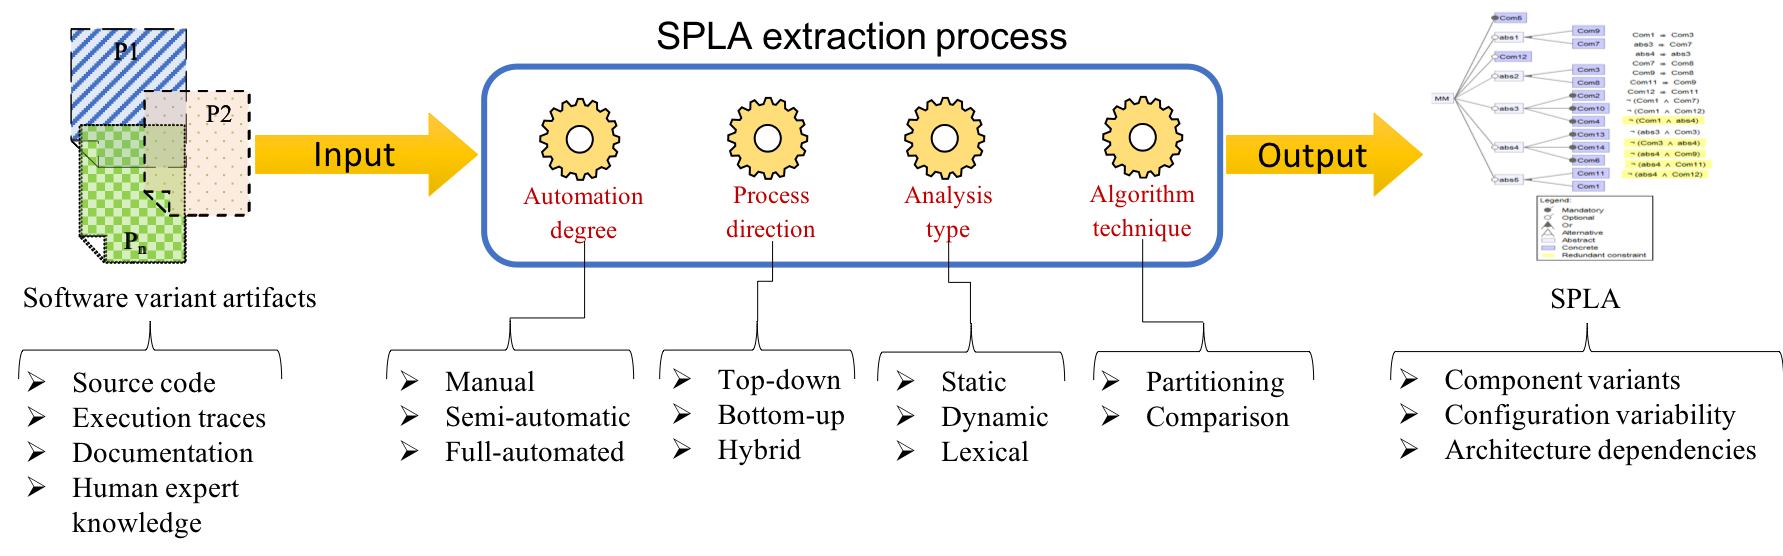
\includegraphics[width=\textwidth]{figs/process-oriented-desing.png}
	\end{center}
	\caption{The good practices of SPLA extraction approach}
	\label{fig:SALife}
\end{figure}

\subsection{The Input Artifacts to be Analyzed for Extracting SPLA}
\index{Input of SPLA extraction}
The input software artifacts of the SPLA extraction approach are used to extract the information related to the variability of software variants and to allow us to recover the SPLA. The input software artifacts can be \textit{source code}, \textit{execution traces}, \textit{documentations} and/or \textit{human expert knowledge}.

\begin{itemize}
	\item \textbf{Source code} is used to determine the functionalities to be implemented by computers. For object-oriented software, the source code consists of classes including methods (e.g., operations) and attributes (e.g, data). The dependencies between classes are method invocations, attribute accesses, inheritance, and so on. All these information allow identifying the variability at the implementation level that reflects the architecture variability. Due to its availability, source code is the most commonly used input artifact to be analyzed by the existing software architecture extraction approaches. These extraction approaches relied on the dependencies between classes to cluster them into disjoint groups representing the component-based architecture (i.e., to identify high cohesive and low coupling partitions) \cite{mende2008supporting,mende2009evaluation,moshkenani2012improving}. \index{Source code analysis}
	
    \item \textbf{Execution traces} represent the system behavior at runtime such that dependencies between software elements are collected during the program execution. They allow one to identify the dynamic variability  between the software variants following different usage scenarios. We can identify these  usage scenarios based on use cases, sequence diagram and test cases \cite{Dugerdil:2013:DDT:2480362.2480602,mishra2009creating,shatnawi2018identifying}. \index{Execution traces}
    
	\item \textbf{Software documentations} include descriptions of the software variants at different level of abstractions \cite{lethbridge2003software}. It can be text-based (e.g., configuration files) or model-based documents (e.g., use cases). We can derive functional components from use cases \cite{shatnawi2018identifying}. Configuration files help to extract information about the previous architecture \cite{Weinreich2012}. Design documents are used to provide information about how components have been designed \cite{kolb2006refactoring}. \index{Documentation}
	
	\item \textbf{Human expert knowledge} is related to persons who have relevant information about the design and the implementation of software variants. Their knowledge can be used to select the main architecture view to be the core of SPLA in \cite{pinzger2004architecture}, and to guide the extraction process by classifying the architectural elements and identifying their dependencies \cite{kang2005feature}. \index{Human expert knowledge}
\end{itemize}


The selection of which input artifacts to be analyzed in the process of SPLA extraction approach is based on: (1) the availability of artifacts, (2) the ease to execute the program, and (3) the decision of software architects.



\subsection{The Process of SPLA Extraction}
\index{Process of SPLA extraction}
The approach process of SPLA extraction aims to analyze the input software artifacts in order to recover the variability of software variants at the architecture level and to identify reusable components composing the recovered SPLA. We see that the process is based on four aspects. These aspects are the \textit{automation degree} of the extraction process, the \textit{direction} of the analysis process, the \textit{type of analysis} to be performed, and the \textit{algorithm} determining the procedure of the process. 

\begin{itemize}

	\item \textbf{The automation degree of the extraction process} refers to the degree in which human expert interactions are required to perform this process. It can be \textit{manual}, \textit{semi-automatic} and \textit{fully-automatic} processes.  \index{Process automation degree}
	
    \begin{itemize}
        \item \textbf{Manual process} totally depends on human experts.  In this context, we provide guides for the experts, such as a visual analysis of the source code that allows identifying architectural elements \cite{langelier2005visualization,22_wu2011recovering}. \index{Manual SPLA extraction}	

        \item \textbf{Semi-automatic process} needs human experts for recommendations to perform the SPLA extraction process \cite{kang2005feature}. Such recommendations are to select the main architecture view to be the core of SPLA \cite{kang2005feature}, to manually analyze design documents \cite{pinzger2004architecture}, and to interact with the approach steps to refine the results \cite{erdemir2011object}. \index{Semi-automatic SPLA extraction}

        \item \textbf{Fully-automated process} does not require human expert interactions to identify SPLA, excluding the need to determine some threshold values \cite{mende2008supporting,shatnawi2017recovering}. \index{Fully-automatic SPLA extraction}

    \end{itemize}

	\item \textbf{The direction of the analysis process} can be \textit{top-down}, \textit{bottom-up} and \textit{hybrid}. \index{Direction of extraction process}
	In top-down, the process analyzes software requirements to extract SPLA. \index{Top-down SPLA extraction} In bottom-up, the process analyzes the source code of software variants to extract SPLA \cite{frenzel2007extending,kang2005feature,koschke2009extending,shatnawi2017recovering}. \index{Bottom-up SPLA extraction}
	Hybrid process refers to the analysis of software requirements (top-down) and source codes (bottom-up) to identify the corresponding software architecture \cite{allier2009identifying}. \index{Hybrid SPLA extraction}
	
	\item \textbf{The type of analysis} to be performed  can be \textit{static}, \textit{dynamic} or \textit{lexical} to identify the relationships between artifacts, in order to to extract SPLA.

    \begin{itemize}
	    \item \textbf{Static analysis} does not require executing software variants to perform the analysis  \cite{pinzger2004architecture,shatnawi2017recovering,Weinreich2012}. We can statically extract graph structures representing the elements (classes, methods, attributes) of the software variants and their related dependencies (calls and references) from the source code \cite{shatnawi2017analyzing}. These graph structures are used to identify the architecture of each software variants and the variability between these identified architectures \cite{pinzger2004architecture,shatnawi2017recovering}. Note that static analysis does not address polymorphism and dynamic binding, and it does not allow to distinguish between the used and unused source code. \index{Static analysis}
	
	    \item \textbf{Dynamic analysis}  {refers to the use of program execution traces to identify the relationships between elements of software variants at the run-time. This allows us to collect actual dependencies between elements. For example, by executing a feature, we can identify software components related to this feature by collecting the executed elements.} However, the limitations against the use of dynamic analysis are: (1) it requires to cope with complex setup of software variants for execution, and (2) the difficulty to identify  all execution scenarios that cover all dependencies in the software variants. To help deal with the second limitations, we can rely on use cases, usage logs and sequence diagrams to identify execution scenarios \cite{Dugerdil:2013:DDT:2480362.2480602,mishra2009creating, shatnawi2018identifying}. \index{Dynamic analysis}

    	\item \textbf{Lexical analysis} relies on the textual information in the software variant artifacts to identify their related dependencies. This analysis supports the identification of cloned functionalities between the software variants \cite{frenzel2007extending,kolb2005case,kolb2006refactoring,koschke2009extending,mende2008supporting,mende2009evaluation}. \index{Lexical analysis}
    \end{itemize}

	\item \textbf{The algorithms that support the extraction process} depend on the formulation of the computational problems of SPLA extraction. The SPLA extraction can be viewed as \textit{partitioning problem} and \textit{comparison problem}.	\index{Algorithms of SPLA extraction}
	
    \begin{itemize}
        \item \textbf{The partitioning problem} aims to recover the software architectures corresponding to all software variants. For this purpose, one can use clustering algorithms \cite{shatnawi2017recovering}, or search-based algorithms \cite{rathee2019multi} to partition classes.
        
        \item \textbf{The comparison problem} aims to identify the variability between these recovered software architectures. Several algorithms can be used like formal concept analysis \cite{carbonnel2017feature,shatnawi2017recovering} and clone detection algorithms \cite{frenzel2007extending,kolb2006refactoring,koschke2009extending} to identify pieces of source code existing in many software variants.
    \end{itemize}
    
\end{itemize}


\section{Illustrative Approach to Extract SPLA}
\label{sec:example-approach}
In this section, we provide example techniques to extract each type of architecture variability of SPLA. We rely on our previous work \cite{shatnawi2017recovering} because it provides techniques that cover all types of architecture variability related to SPLA. 

\subsection{Input and Goal}

For simplicity, let us consider that we have as input the component-based architecture of each single software variant. Each component-based architecture is a set of disjoint groups of classes such that each group of classes represents the implementation of a component in this architecture. This component-based architecture can be extracted based on any architecture recovery approach by analyzing the object-oriented source code of each single software variant. A comprehensive survey of these approaches coud be found at~\cite{abdellatiftaxonomy,ducasse2009software,lima2017investigating}. 

The goal is to find the commonality and variability between the component-based architectures respectively recovered from each single software variants. This is based on: (1) the extraction of component variability including the component variants and their related structure and interface variability, and (2) the extraction of configuration variability including the component existence variability, component-to-component link variability, and component dependencies.

\subsection{Extraction of Component Variability}
\index{Extraction of component variability}
\subsubsection{Extraction of Component Variants}
\index{Extraction of component variants}
Component variants are extracted based on the identification of components providing the same, or at least similar, core functionalities. Since that these functionalities are implemented based on the object-oriented source code, a group of components sharing the majority of their source code is considered as components providing similar functionalities. Software architects should define the similarity degree to consider this group of components to be components variants.

Textual analysis allows identifying the semantic relationships between the classes of different components. 
Each component is seen as a text document that contains the implementation of classes composing this component.
Then, a text-based clustering algorithm is used to identify similar components that are considered as component variants of the same architectural element. 
Note that two components from the same software variant should not be grouped together in the same cluster. The clustering algorithm should adhere to this condition to forbid this situation.

\subsubsection{Extraction of Component Structure Variability}
\index{Extraction of component structure variability}
At this stage, the source code of component variants is used to extract their structure variability in terms of common and variable classes.
Formal Concept Analysis (FCA) allows one to identify common and variable classes as well as the distribution of variable classes in the component variants. The formal context of FCA considers component variants and classes as objects and attributes respectively. The objects of this formal context have attributes based on the classes distribution in the implementation of the corresponding component variants. We give an example of a formal context of three component variants in Table \ref{FCcomVar} where X refers to that the \textit{variant} includes the corresponding \textit{class} in its implementation. Then, FCA generates a \textit{lattice} based on this formal context that is presented in Figure \ref{fig:lattComVar}. Following this lattice, the common classes are grouped in the root node of the lattice, while the variable ones are distributed in other nodes. A component variant has all classes included in all nodes placed in the path to the root node.

\begin{table}[h]
 \centering
 \caption{An example of formal context of three component variants}
 \resizebox{\textwidth}{!}{
 \label{FCcomVar}
\begin{tabular}{|l|l|l|l|l|l|l|l|l|}
\hline
\textbf{} & CD & Reader & Transformer & StreamManager & Helper & Writer & Encoder & Decoder \\ \hline
Variant 1 & X & X & X & X & X &  &  & X \\ \hline
Variant 2 & X & X & X & X & X & X &  &  \\ \hline
Variant 3 & X & X & X & X &  &  & X & X \\ \hline
\end{tabular}
}
\end{table}

\begin{figure}[h]
\centering
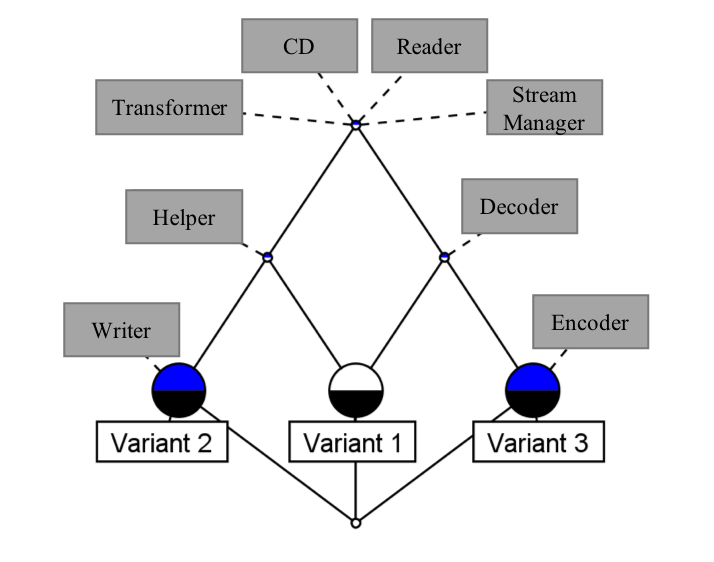
\includegraphics[width=0.7\textwidth]{figs/component_variant_lattice.png}
\caption{A lattice example of three component variants}
\label{fig:lattComVar}
\end{figure}

\subsubsection{Extraction of Component Interface Variability}
\index{Extraction of component interface variability}
Now that the structure variability is extracted, the next step is to  extract the mandatory and optional interfaces of component variants. The interfaces of each component variant are identified as they are structured in the corresponding software variant where the component variant has been extracted. One can use any approach of Seriai et al. \cite{seriai2014deriving} or Lui et al. \cite{liu2018component} to extract groups of methods representing the component interfaces. 
The textual analysis allows one to identify the semantic similarity between interfaces of component variants to determine similar interfaces. This textual analysis compares the methods of each interface with ones of other interfaces based on the header and body of methods. Software architects can use a pre-defined threshold similarity value to decide whether interfaces are similar or not. Once similar interfaces are detected in the different variants of a component, the intersection determines the mandatory interfaces. The remaining ones are optional interfaces.  


\subsection{Extraction of Configuration Variability}
\index{Extraction of configuration variability}

\subsubsection{Extraction of Component Existence Variability}
\index{Extraction of component existence variability}

Formal Concept Analysis (FCA) is also used to analyze the component existence variability. In the formal context, each software architecture of a software variant is represented in terms of an object that has a set of components as attributes. FCA generates a lattice of concepts representing the distribution of the components in the different architectures. Based on this lattice, the mandatory components are grouped in the root node of the lattice, while the variable components are in the other nodes.

In Figure \ref{fig:lattArchExam}, we provide an example of a lattice for architectures of three software variants related to to our illustrative example of the audio player famility presented in Figure \ref{fig:archVarExam1}. The mandatory components are \textit{CD Reader}, \textit{Sound Source} and \textit{Player}, and the optional components are \textit{Remote Control}, \textit{MP3 Decoder}, \textit{Purchase Reminder}, \textit{MP3 Decoder}, \textit{Login} and \textit{Alarm}.

\begin{figure}[h]
\centering
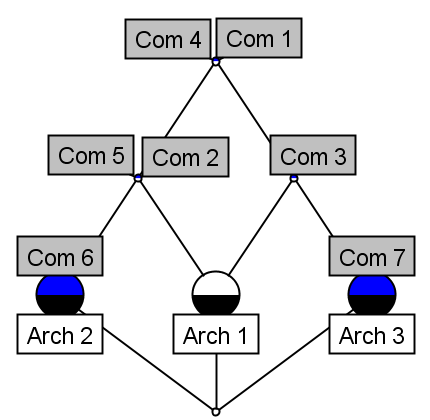
\includegraphics[scale=0.75]{figs/FCA_Arhc_Exam.png}
\caption{A lattice example of three architectural configurations}
\label{fig:lattArchExam}
\end{figure}


\subsubsection{Extraction of Component-to-component Link Variability}
\index{Extraction of component-to-component link variability}
For each component, the set of components that have links with this component in each software variant are identified. The mandatory component-to-component links are identified based on the intersection between the links of this component in different software variants. The other component-to-component links are optional ones.


\subsubsection{Extraction of Component Dependencies}
\index{Extraction of component dependencies}
The identification of dependencies between optional components is done using the same lattice generated by FCA in Figure \ref{fig:lattArchExam}. The intent of each node in this lattice contains a group of components (e.g. \textit{MP3 Decoder} and \textit{Remote Control}) and the extent  of each node is a group of architectural configurations (e.g. \textit{Arch 2}).
The architecture configurations can be reverse-engineered from this lattice based on paths identified starting from their nodes to the root of the lattice. Each path consists of an ordered series of nodes. This order is based on the hierarchical distribution of the nodes called sub-concept to super-concept relationships.

The process to extract these paths consists of two steps as follows. 

\begin{enumerate}
    \item \textbf{Node numbering} is based on the \textit{Breadth First Search (BFS)} algorithm \cite{cormen2009introduction}. BFS helps extracting a tree-based representation from the lattice starting from its root node. BFS will visit the nodes at distance \textit{1}, then it will visit the nodes at distance 2 and so on. Figure \ref{fig:BFSexample} shows the steps of BFS for numbering nodes. The number of a node denotes to the distance of visiting a given node and $\infty$ refers to unvisited nodes. 
    
    \item \textbf{Path extraction} starts from each node holding an extent (e.g. \textit{Arch 1}). It goes in a bottom-up direction based on the numbers identified in the previous step to nodes having a lower numbering. It performs this process recursively until reaching the root node that has \textit{0} numbering. We provide in Figure \ref{fig:FCA_Arch_Path} the three paths identified based on our example in Figure \ref{fig:lattArchExam}. These three paths are respectively presented by solid, dashed and double dashed arrows. For example, the path corresponding to \textit{Arch 1} includes the node of \textit{Login}, the node of \textit{MP3 Decoder} and \textit{Remote Control} and the node of \textit{CD Reader} \textit{Sound Source}, and \textit{Player}.
\end{enumerate}

\begin{figure} [h]
\centering
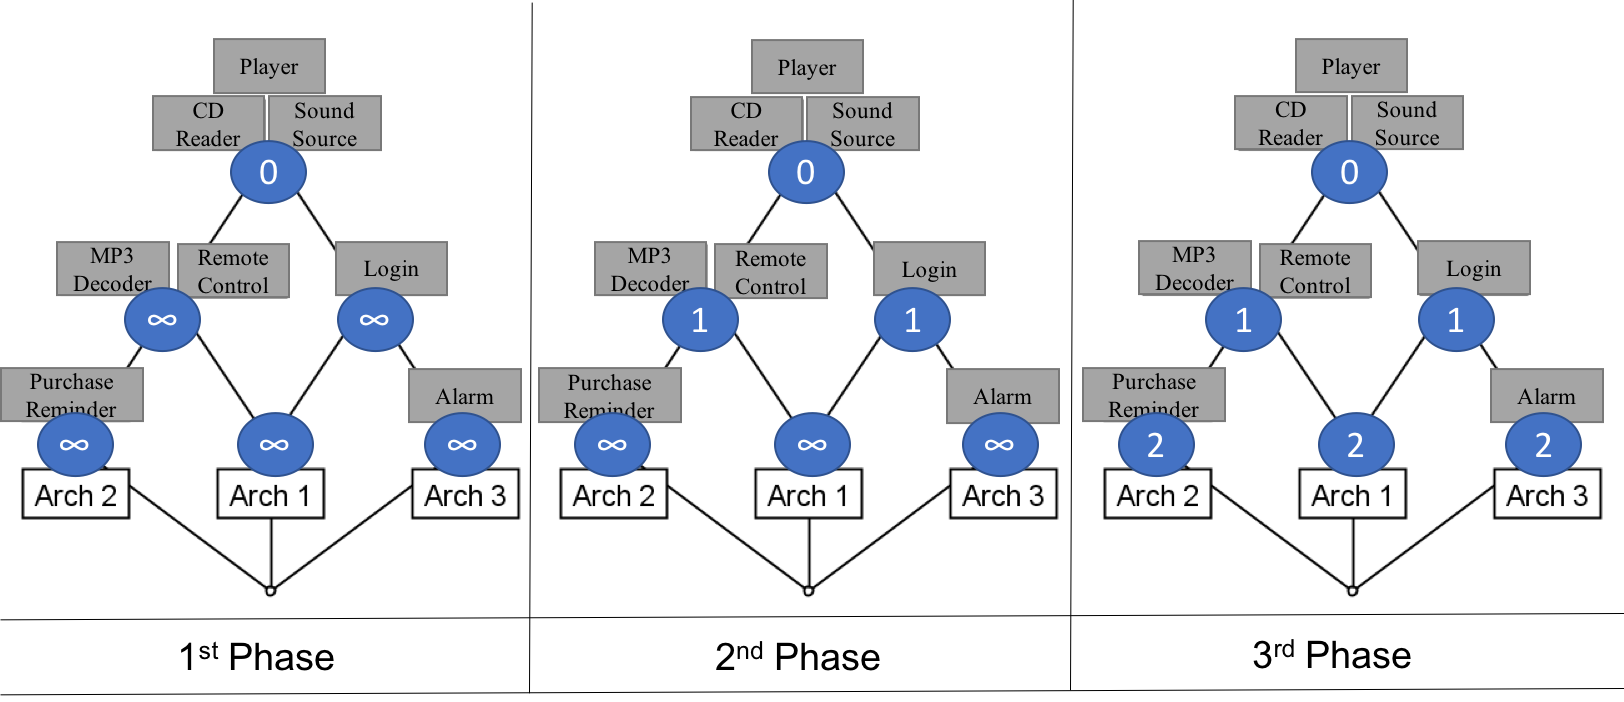
\includegraphics[width=\textwidth]{figs/bfsExample.png}
\caption{An example of BFS process}
\label{fig:BFSexample}
\end{figure}


\begin{figure} [h]
\centering
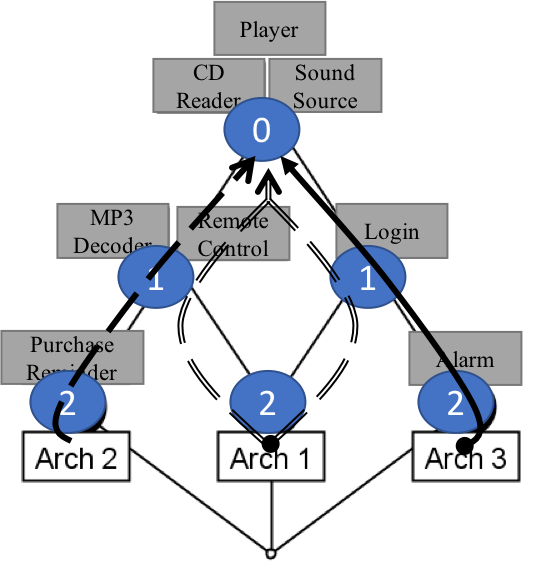
\includegraphics[width=0.5\textwidth]{figs/FCA_Arch_path.png}
\caption{An example of paths extracted from FCA lattice}
\label{fig:FCA_Arch_Path}
\end{figure}

The next process is to extract the dependencies between components based on these identified paths.


\begin{itemize}

\item \textbf{Required dependency extraction.} It is based on \textit{parent-to-child relationships} between the nodes. A node requires another node if this node appears after the other node in all of the identified paths. Due to the sub-concept and the super-concept between these nodes, the first node cannot be reached without passing the required node in the lattice. Considering our example in Figure \ref{fig:lattArchExam}, \textit{Purchase Reminder} requires \textit{Remote Control} and \textit{MP3 Decoder}. \index{Extraction of Required dependencies}


\item \textbf{Exclude dependency extraction.} It is based on the identification of nodes that do not have any sub-concept to super-concept relationship in all paths.  Two nodes are considered having exclude dependency if they never appear together in all paths. Considering our example in Figure \ref{fig:lattArchExam}, \textit{Purchase Reminder} and \textit{Alarm} exclude each other as they never appear together in paths identified in Figure \ref{fig:FCA_Arch_Path}. \index{Extraction of Exclude dependencies}

\item \textbf{Alternative dependency extraction.} It is the generalized form of the exclude one by exclusively choosing one component from a group of components having the alternative dependencies between each other. Therefore, the identification of alternative dependency is based on a group of nodes that hold exclude dependency with each node in this group. This is based on the set cover extraction algorithm from the graph theory \cite{cormen2009introduction}.  {For example, if node \textit{A} is excluded with nodes \textit{B} and \textit{C} on the one hand, and node \textit{B} is excluded with node \textit{C} on the other hand, then the group of \textit{A, B} and \textit{C} forms an alternative dependency.} \index{Extraction of Alternative dependencies}

\item \textbf{And dependency extraction.} It is based on a group of components grouped in the same node in the lattice. \textit{Remote Control} and \textit{MP3 Decoder} have an And dependency in our example in Figure \ref{fig:lattArchExam}. \index{Extraction of And dependencies}


\item \textbf{Or dependency extraction.}  {When some components are concerned by an OR dependency, this means that at least one of them should be selected; i.e., the architectural configuration may contain any combination of these components. Therefore, in the case of absence of other dependencies any pair of components is concerned by an OR dependency. Thus, pairs concerned by required, exclude, alternative, or AND dependencies are ignored as well as those concerned by transitive require dependencies; e.g., \textit{Purchase Reminder} and \textit{Alarm} are ignored since they are exclusive.\\
The process of identifying the OR groups is as follows. Firstly, we check the dependencies between each pair of nodes. Pairs that have required, exclude, alternative, and AND dependencies are ignored. All pairs having transitive require dependencies are also ignored. The reason of the exclusion is that these dependencies break the OR one. Then, the remaining pairs of nodes are assigned an OR dependency. Next, we analyze these pairs by testing the dependency of their nodes. Pairs sharing a node need to be resolved (e.g., in Figure \ref{fig:lattArchExam}, a pair of \textit{MP3 Decoder}-\textit{Remote Control} and \textit{Alarm}, and a pair of \textit{MP3 Decoder}-\textit{Remote Control} and \textit{Login}, where \textit{MP3 Decoder}-\textit{Remote Control} is a shared node). The resolution is based on the dependency between the other two nodes (e.g., \textit{Login} and \textit{Alarm}). If these nodes have a require dependency, then we select the highest node in the lattice (i.e., the parent causes the OR dependency to its children). If the dependency is excluded or alternative one, then we remove all OR dependencies (i.e., an exclude dependency violates an OR one). In the case of sharing an OR dependency, the pairs are grouped to one OR dependency. AND dependency will not occur in this case according to the AND definition.}

\index{Extraction of groups of variability}
\item \textbf{Extraction of groups of variability} aims to identify dependencies among groups of dependencies. Since an AND group can be considered as one coherent entity, it is not allowed for its components to partially have internal dependencies, e.g. dependent through an OR with other groups. This implies that all components belonging to an AND group should have the dependency.
For alternative and OR dependencies, it is allowed to take AND ones as a member. In addition, the internal dependencies between alternative and OR dependencies are allowed. In other words, an alternative dependency can be a member of an OR dependency and vice versa. 
According to that, the AND dependency has a high priority to be added before the others while OR and alternative have the same priority.
The identification of the hierarchical tree starts from the root of the tree by directly connecting all mandatory components to it  {(e.g., \textit{CD Reader}, \textit{Sound Source} and \textit{Player})}. At this stage, the tree does not have a hierarchy. Then, optional components are added based on their relationships. Groups of components having AND dependencies are added by creating an abstract node that carries out these components  {(e.g., \textit{Remote Control} and \textit{MP3 Decoder} are added using a group of an AND dependency)}. The relation between the parent and the children is an AND dependency. Next, alternative dependencies are represented by an abstract node that carries out these components (\textit{Purchase Reminder} and \textit{Alarm}). Next, OR dependencies are applied by adding an abstract node as a parent to components having an OR. In the case where the relation is between a set of components having AND dependency as well as alternative dependency, the connection is made with their abstract nodes (i.e. the abstract nodes corresponding to the AND dependency and the alternative one become children of the OR parent). Next, the remaining components are directly added to the root with optional notation. Finally, the cross-tree dependencies are added (i.e. required and exclude ones). 

{In Figure \ref{fig:audio-arch-feature-model}, we present the architecture variability related to the dependencies between components of the audio player software family presented in Figure \ref{fig:archVarExam1}}
\end{itemize} 

{For more details regarding the approach and the evaluation results, please refer to \cite{shatnawi2017recovering}.}


\begin{figure} [h]
\centering
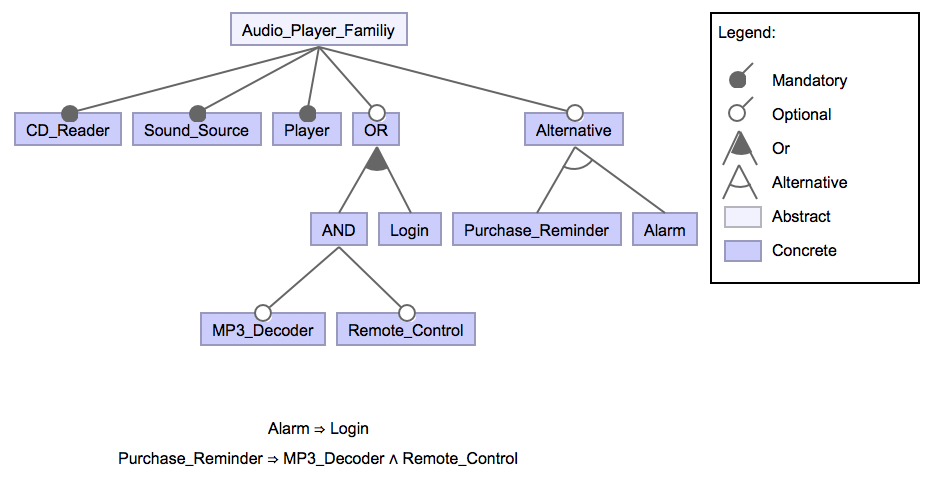
\includegraphics[width=0.85\textwidth]{figs/audio-player-arch-fm.png}
\caption{The resulting component dependencies in terms of feature modeling representation of the illustrative example presented in Figure \ref{fig:archVarExam1}}
\label{fig:audio-arch-feature-model}
\end{figure}



\section{Conclusion}
\label{sec:conclusion}
To support the reengineering of existing software variants into SPLs, 
we discussed in this chapter the extraction of the Software Product Line Architecture (SPLA) based on the analysis of several software variants. We defined the different types of architecture variability of SPLA elements including component variability, configuration variability and dependencies between components. 

We analyzed the-state-of-the-art of architecture extraction to identify good practices related to the extraction of SPLA. We found that the input artifacts of a  SPLA extraction approach could be source code, execution traces, documentations and human expert knowledge. The processes used to analyze these input artifacts are based on several automation degrees, directions, analysis types to be performed, and the algorithms determining the procedure of the process.
 

As examples of the implementation of some good practices, we presented an illustrative approach for extracting SPLA based on the analysis of many software variants using Formal Concept Analysis. This approach identifies mandatory and optional components as well as the dependencies among components and draw them in terms of Feature Modeling language.
However, this illustrative approach is sensitive to the input software variants as dependencies between components are identified based on component occurrences in the software architectures of these software variants. To cope with this sensitivity, we suggest to carefully select software variants covering a large number of dependencies. Also, to improve the resulting SPLA, we recommend to rely on other software artifacts such as documentations and feature models.

As future directions, we recommend researchers consider the evaluation of the different good practices presented in this chapter, in order to identify best combinations and configurations of these good practices that maximize the accuracy of a SPLA extraction approach. 

%
% Bibliography sample
\bibliographystyle{spmpsci}
\bibliography{ExSPLArch}

% Commented out ...
%\input{referenc}

\printindex

\end{document}
